\begin{problem}[习题2.6]右图的无向图以邻接链表存储,
\vspace{-2em}
\begin{multicols}{2}
~

而且在关于每个顶点的链表中与该顶点相邻的顶点是按照字母顺序排列的.
试以此图为例描述讲义中算法DFNL的执行过程.

\begin{center}
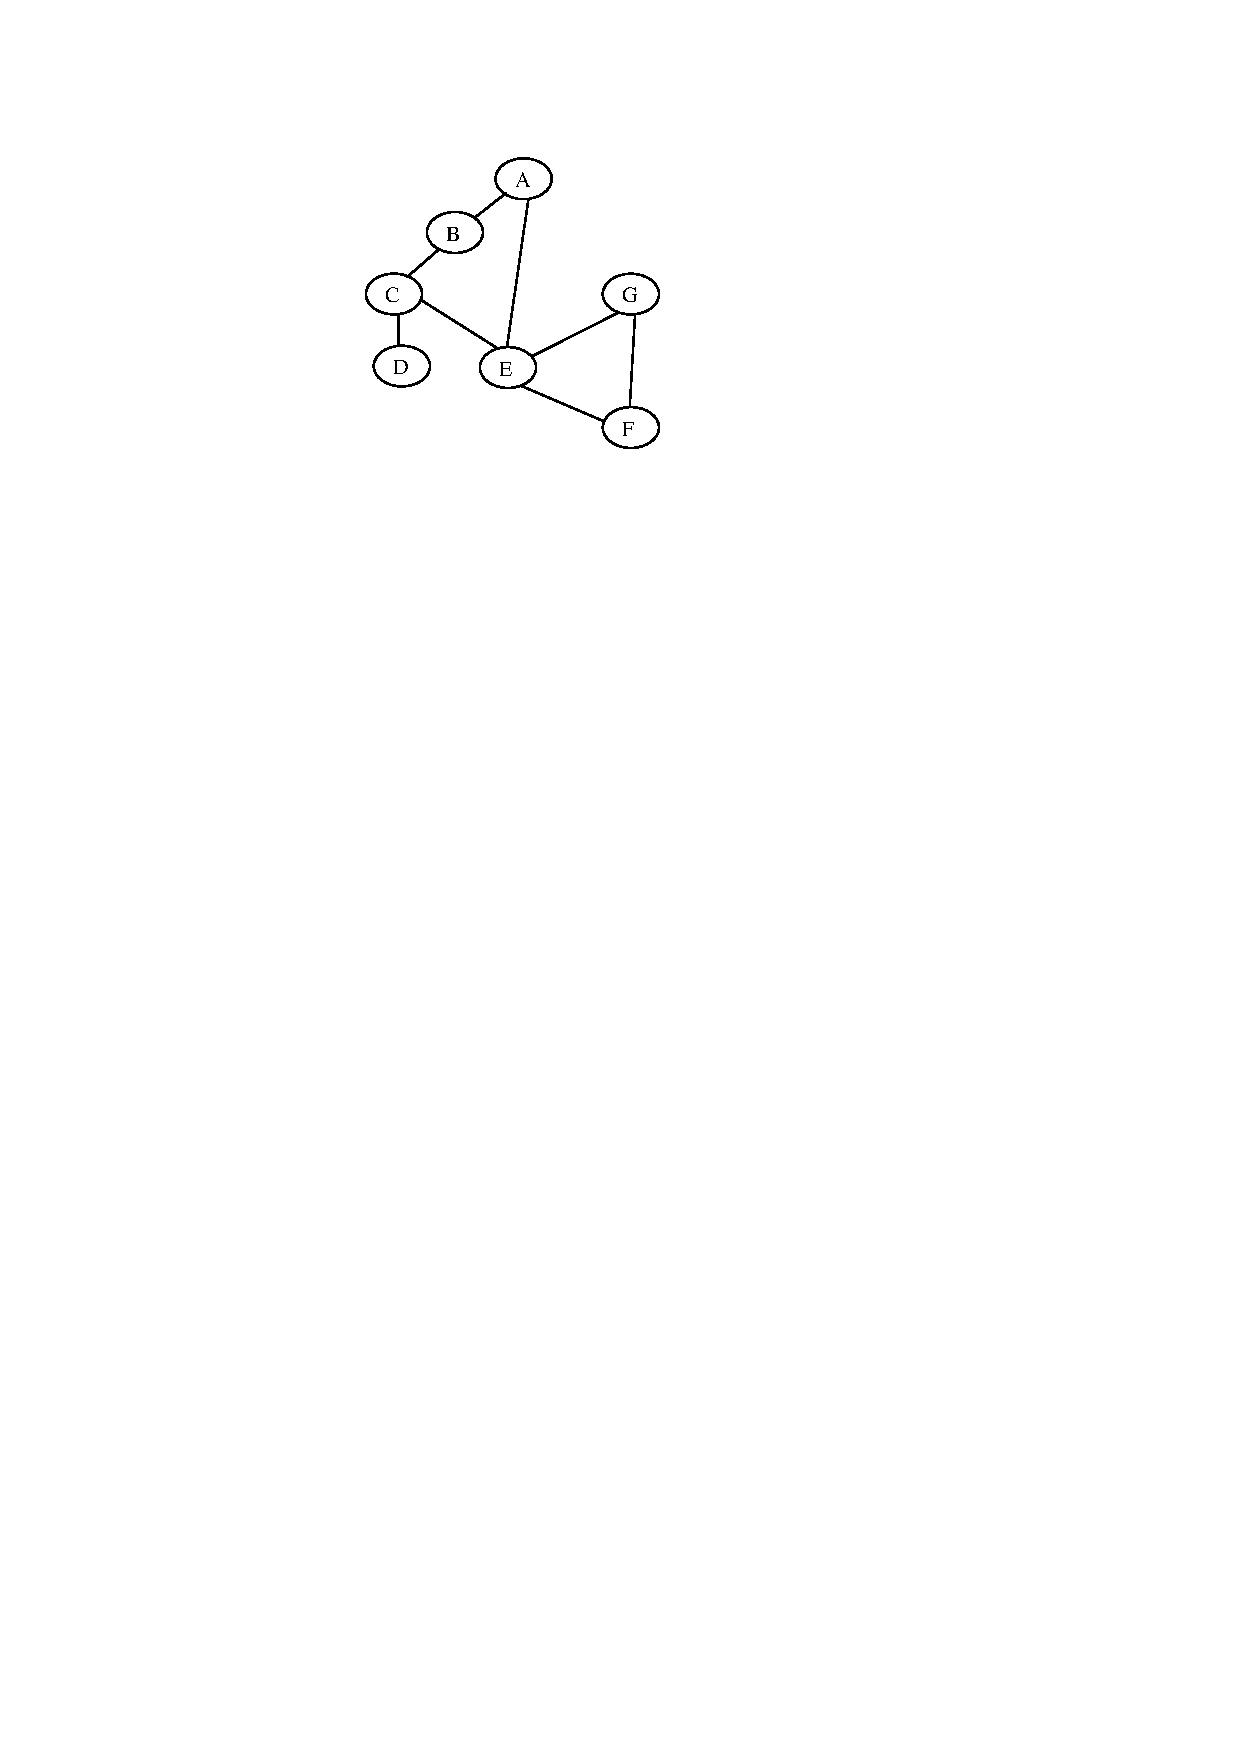
\includegraphics[width=0.12\textwidth]{fig01.pdf}\\
一个无向图$G$
\end{center}

\end{multicols}

\end{problem}
\begin{solution}
\textbf{解:}题中所给的无向图所对应的邻接链表如图\ref{link}所示.
\begin{figure}[!htb]
\centering
\begin{tabular}{l|l|l|l|l|l|l|l|llllll}
\cline{2-2}\cline{4-5}\cline{7-8}
A & { ~ } & $\rightarrow$ & B &  & $\rightarrow$ & E & 0 &  &  &  &  &  &  \\
\cline{2-2}\cline{4-5}\cline{7-8}
B &  & $\rightarrow$ & A &  & $\rightarrow$ & C & 0 &  &  &  &  &  &  \\
\cline{2-2}\cline{4-5}\cline{7-8}\cline{10-11}
C &  & $\rightarrow$ & B &  & $\rightarrow$ & D &  & \multicolumn{1}{l|}{$\rightarrow$} & \multicolumn{1}{l|}{E} & \multicolumn{1}{l|}{0} &  &  &  \\
\cline{2-2}\cline{4-5}\cline{7-8}\cline{10-11}
D &  & $\rightarrow$ & C & 0 & \multicolumn{1}{l}{} & \multicolumn{1}{l}{} & \multicolumn{1}{l}{} &  &  &  &  &  &  \\
\cline{2-2}\cline{4-5}\cline{7-8}\cline{10-11}\cline{13-14}
E &  & $\rightarrow$ & A &  & $\rightarrow$ & C &  & \multicolumn{1}{l|}{$\rightarrow$} & \multicolumn{1}{l|}{F} & \multicolumn{1}{l|}{} & \multicolumn{1}{l|}{$\rightarrow$} & \multicolumn{1}{l|}{G} & \multicolumn{1}{l|}{0} \\
\cline{2-2}\cline{4-5}\cline{7-8}\cline{10-11}\cline{13-14}
F &  & $\rightarrow$ & E &  & $\rightarrow$ & G & 0 &  &  &  &  &  &  \\
\cline{2-2}\cline{4-5}\cline{7-8}
G &  & $\rightarrow$ & E &  & $\rightarrow$ & F & 0 &  &  &  &  &  &  \\
\cline{2-2}\cline{4-5}\cline{7-8}
\end{tabular}
\caption{\label{link}无向图的邻接链表}
\end{figure}
此图讲义中算法DFNL的执行过程如下:\\
{\small
\begin{tabular}{lllllll}
\multicolumn{7}{l}{初始化  数组DFN:=0,  num=1;} \\
 & \multicolumn{6}{l}{A为树的根节点,对A计算DFNL(A,null), DFN(A):=num=1; L(A):=num=1; num:=1+1=2.} \\
 & \multicolumn{6}{l}{从邻接链表查到A的邻接点B,} \\
 &  & \multicolumn{5}{l}{因为DFN(B)=0,对B计算DFNL(B,A), DFN(B):= num=2; L(B):=num=2; num:=2+1=3.} \\
 &  & \multicolumn{5}{l}{查邻接链表得到B的邻接点A, 因为DFN(A)=1 0, 但A=A, 即是B的父节点,无操作.} \\
 &  & \multicolumn{5}{l}{接着查找邻接链表得到B的邻接点C,因为DFN(C)=0,} \\
 &  &  & \multicolumn{4}{l}{对C计算DFNL(C,B), DFN(C):= num=3;  L(C):=num=3; num:=3+1=4.} \\
 &  &  & \multicolumn{4}{l}{查找C的邻接点B,因为DFN(B)=1≠0, 但B=B,即是C的父节点, 无操作.} \\
 &  &  & \multicolumn{4}{l}{接着查找邻接链表得到C的邻接点D,因为DFN(D)=0,} \\
 &  &  &  & \multicolumn{3}{l}{对D计算 DFNL(D,C), DFN(D):= num=4;   L(D):=num=4;  num:=4+1=5.} \\
 &  &  &  & \multicolumn{3}{l}{查找得D邻接点C,而DFN(C)=3≠0,但C=C,为D的父节点, L(D)保持不变.} \\
 &  &  &  & \multicolumn{3}{l}{D的邻接链表结束,DFNL(D,C)的计算结束.} \\
 &  &  & \multicolumn{4}{l}{返回到D的父节点C,查找邻接链表得到C的邻接点E, 因为DFN(E)=0,} \\
 &  &  &  & \multicolumn{3}{l}{对E计算DFNL(E,C), DFN(E):=num=5;   L(E):=num=5;   num:5+1=6;} \\
 &  &  &  & \multicolumn{3}{l}{查找得E邻接点A,因DFN(A)=1≠0,又A≠C,变换L(E)=min(L(E), DFN(A))=1.} \\
 &  &  &  & \multicolumn{3}{l}{查找得E邻接点C,因DFN(C)=3≠0,但C=C,无操作.} \\
 &  &  &  & \multicolumn{3}{l}{查找得E邻接点F, 因DFN(F)=0,} \\
 &  &  &  &  & \multicolumn{2}{l}{对F计算 DFNL(F,E), DFN(F):=num=6;   L(F):=num=6;  num:=6+1=7;} \\
 &  &  &  &  & \multicolumn{2}{l}{查找得F邻接点E,因DFN(E)=5≠0,但E=E,无操作.} \\
 &  &  &  &  & \multicolumn{2}{l}{查找得F邻接点G,因DFN(G)=0,} \\
 &  &  &  &  &  & 对G计算 DFNL(G,F),DFN(G):=num=7;   L(G):=num=7;  num=7+1=8; \\
 &  &  &  &  &  & 查找G邻接点E,因DFN(E)=5≠0,又E≠F,L(G)=min(L(G),DFN(E))=5 \\
 &  &  &  &  &  & 查找得G邻接点F,因DFN(F)=6≠0,但F=F,无操作. \\
 &  &  &  &  &  &  G的邻接链表结束,DFNL(G,F)的计算结束. \\
 &  &  &  &  &  & L(F):=min(L(F),L(G))=min(6,5)=5 \\
 &  &  &  &  & \multicolumn{2}{l}{F的邻接链表结束,DFNL(F,E)的计算结束.} \\
 &  &  &  &  & \multicolumn{2}{l}{L(E):=min(L(E),L(F))=min(1,5)=1} \\
 &  &  &  & \multicolumn{3}{l}{E邻接链表结束, DFNL(E,C)计算结束.} \\
 &  &  &  & \multicolumn{3}{l}{L(C):=min(L(C),L(E))=min(3,1)=1} \\
 &  &  & \multicolumn{4}{l}{C的邻接链表结束,DFNL(C,B)计算结束.} \\
 &  &  & \multicolumn{4}{l}{L(B):=min(L(B),L(C))=min(2,1)=1} \\
 &  & \multicolumn{5}{l}{查找B的邻接链表结束,DFNL(B,A)计算结束.} \\
 &  & \multicolumn{5}{l}{L(A):=min(L(A),L(B))=1} \\
 & \multicolumn{6}{l}{查找得A的邻接点E,因DFN(E)=0,又E≠null,则L(A)=min(L(A),DFN(E))=1} \\
\multicolumn{7}{l}{查找A的邻接链表结束,DFNL(A,null)计算结束.} \\
\end{tabular}
}

\end{solution}
